\documentclass[tikz,border=4pt]{standalone}
\usepackage[T1]{fontenc}
\usepackage{amsmath,amssymb,booktabs}
\usepackage{pgfplots}
\usepackage{pgfplotstable}
\usepackage{xcolor}
\usetikzlibrary{arrows.meta,positioning,fit,backgrounds}
\usepgfplotslibrary{fillbetween,groupplots}
\pgfplotsset{compat=1.18}
\definecolor{paperbg}{HTML}{F6F2EA}
\definecolor{panelbg}{HTML}{FBF8F2}
\definecolor{ink}{HTML}{1E2430}
\definecolor{gridline}{HTML}{D7D0C4}
\definecolor{baseblue}{HTML}{0072B2}
\definecolor{variantorange}{HTML}{D55E00}
\definecolor{altgreen}{HTML}{009E73}
\definecolor{gold}{HTML}{CC9C2C}
\definecolor{slate}{HTML}{4E5A6A}
\pagecolor{paperbg}
\color{ink}
\pgfplotsset{
  every axis/.append style={
    axis line style={draw=gridline},
    tick style={draw=gridline},
    tick label style={color=ink},
    label style={color=ink},
    title style={color=ink},
    grid=major,
    grid style={draw=gridline, line width=0.3pt},
    minor grid style={draw=gridline!60, line width=0.2pt},
    legend cell align=left,
    legend style={draw=none, fill=none, font=\small},
    clip mode=individual,
  }
}

\begin{document}
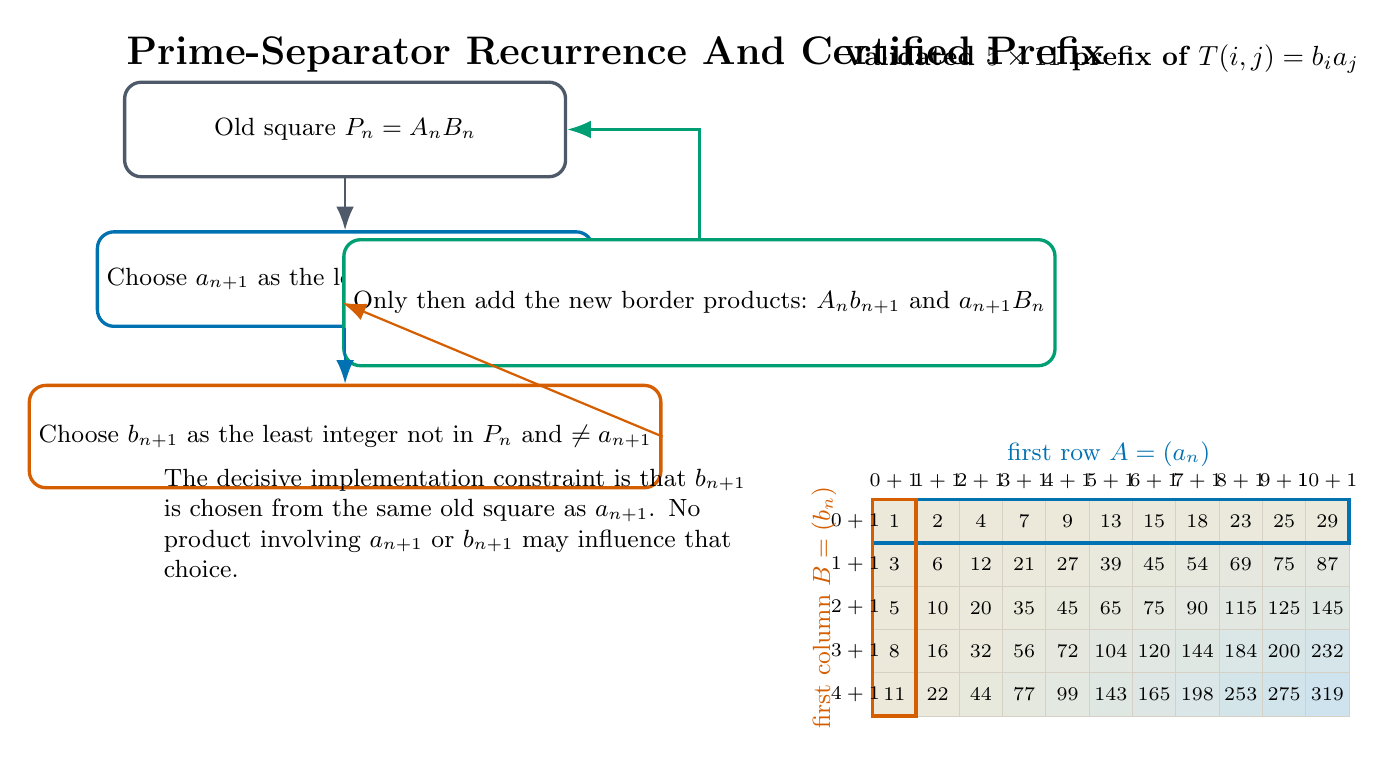
\begin{tikzpicture}[font=\small]
  \node[anchor=north west,font=\bfseries\Large] at (0,6.2) {Prime-Separator Recurrence And Certified Prefix};

  \node[draw=slate, very thick, rounded corners=6pt, fill=white, minimum width=5.6cm, minimum height=1.2cm, align=center] (p) at (2.9,4.9) {Old square $P_n=A_nB_n$};
  \node[draw=baseblue, very thick, rounded corners=6pt, fill=white, minimum width=5.6cm, minimum height=1.2cm, align=center] (a) at (2.9,3.0) {Choose $a_{n+1}$ as the least\ integer not in $P_n$};
  \node[draw=variantorange, very thick, rounded corners=6pt, fill=white, minimum width=5.6cm, minimum height=1.3cm, align=center] (b) at (2.9,1.0) {Choose $b_{n+1}$ as the least\ integer not in $P_n$ and $\neq a_{n+1}$};
  \node[draw=altgreen, very thick, rounded corners=6pt, fill=white, minimum width=5.3cm, minimum height=1.6cm, align=center] (u) at (7.4,2.7) {Only then add the new border products:\ $A_n b_{n+1}$ and $a_{n+1} B_n$};
  \draw[-{Latex[length=3mm]},thick,slate] (p) -- (a);
  \draw[-{Latex[length=3mm]},thick,baseblue] (a) -- (b);
  \draw[-{Latex[length=3mm]},thick,variantorange] (b.east) -- (u.west);
  \draw[-{Latex[length=3mm]},thick,altgreen] (u.north) |- (p.east);
  \node[align=left,text width=7.4cm] at (4.3,-0.1) {The decisive implementation constraint is that $b_{n+1}$ is chosen from the same old square as $a_{n+1}$. No product involving $a_{n+1}$ or $b_{n+1}$ may influence that choice.};

  \begin{scope}[shift={(9.6,0.2)}]
    \node[font=\bfseries] at (2.9,5.6) {Validated $5\times11$ prefix of $T(i,j)=b_i a_j$};
    \foreach \r/\vals in {
      0/{1,2,4,7,9,13,15,18,23,25,29},
      1/{3,6,12,21,27,39,45,54,69,75,87},
      2/{5,10,20,35,45,65,75,90,115,125,145},
      3/{8,16,32,56,72,104,120,144,184,200,232},
      4/{11,22,44,77,99,143,165,198,253,275,319}}
    {
      \foreach \v [count=\c from 0] in \vals {
        \pgfmathsetmacro{\shade}{20+75*(\v/319)}
        \fill[baseblue!\shade!gold!20] (0.55*\c,-0.55*\r) rectangle +(0.55,-0.55);
        \draw[gridline] (0.55*\c,-0.55*\r) rectangle +(0.55,-0.55);
        \node[font=\scriptsize] at (0.55*\c+0.275,-0.55*\r-0.275) {\v};
      }
    }
    \draw[baseblue,very thick] (0,0) rectangle +(6.05,-0.55);
    \draw[variantorange,very thick] (0,0) rectangle +(0.55,-2.75);
    \foreach \c in {0,...,10} {\node[font=\scriptsize] at (0.55*\c+0.275,0.23) {$\c+1$};}
    \foreach \r in {0,...,4} {\node[font=\scriptsize] at (-0.22,-0.55*\r-0.275) {$\r+1$};}
    \node[baseblue,font=\small] at (3.0,0.58) {first row $A=(a_n)$};
    \node[variantorange,font=\small,rotate=90] at (-0.62,-1.37) {first column $B=(b_n)$};
  \end{scope}
\end{tikzpicture}
\end{document}
